\chapter{A simple implementation}
\label{chapter3}
\thispagestyle{empty}

\noindent First, we set up the necessary entities to implement \textit{Sticky Policies}: an Android client and a service provider. The client was developed using Android Studio and emulated through the Android Emulator with a Nexus 5X device running Android 7.0 and API level 24. The Trusted Authority was developed using Eclipse and run on Apache Tomcat 8; the communication was implemented through HTTP protocol.

The app was also tested in a Samsung tablet (SM-T230) running Android 4.4.2 and API level 19, to test performance on a real device with lower level API and operating system, together with a different screen dimension.

In this solution, \textit{Sticky Policies} are realized via XML files and paired with personal data through the combination of symmetric and asymmetric cryptography. This approach is presented in \cite{pearson2011sticky}, and an example XML policy was created taking as a reference the one presented in the same paper. Following this specification, we present a protocol for the communication of two Android clients, called for simplicity Alice and Bob. 

Alice generates an XML policy to regulate data access, encrypting it with a symmetric key generated locally. The policy and the keys are then encrypted with the Trusted Authority's public key and signed by Alice. Purposely, Alice should obtain the public key of the Trusted Authority and also a key pair for herself: in our solution, we use self-signed X509 Certificates generated by combining the Java Cryptography Architecture and the Bouncy Castle cryptography APIs for Java. Alice thus contacts the Trusted Authority to obtain its public key, and shares her own if the Trusted Authority is not the issuer of the certificate itself.

Bob obtained Alice's encrypted data and an attached policy in clear text, together with other encrypted data to guarantee integrity, confidentiality and non-refusal of the policy and data. To decrypt Alice's data, he must follow these steps:
\begin{itemize}
	\item Bob asks the Trust Authority to release the symmetric key, presenting the encrypted data signed by Alice.
	\item The Trust Authority evaluates the policy and Bob's reliability, submitting some challenges for him to complete.
	\item If trusted, Bob receives the symmetric key to decrypt Alice's personal data.
\end{itemize}

Data is exchanged through POST requests over a channel which is assumed to be secure.

Once the Trust Authority receives a request from the client, it checks the correct specification of the policy before proceeding to decrypt and verify the payload received. This operation is performed by a server-side parser which matches the XML file with a standard XSD grammar. In case of errors, no symmetric key is released.

The specification of the XSD grammar can be found in Appendix \ref{appendixA}. 

\section{Program flow and architecture}
implementation of the protocol, insert some images
add error management
lifecycle considerations
check manifest permissions: storage??

We start by analysing the application flow before that data is shared, given that Alice has installed an instance of the StickyPolicyApp.

The data owner can either share a simple text message (shown in Figure \ref{fig:share-text}) or a regular file inside his phone (for example, an image, in Figure \ref{fig:share-img}), chosen through a picker. Consequently, the underlying application generates a fitting policy depending on the data shared and on the owner itself, which is then passed on to the next \texttt{Activity} for encryption and sharing. In this solution, for the sake of simplicity, the generated policy contains mock data, except for the X509 Certificate serial number and the data type. Possible future works include adding an interactive policy generator to allow the user to define sharing constraints.
\begin{figure}
	\centering
	\begin{minipage}{0.35\textwidth}
		\centering
		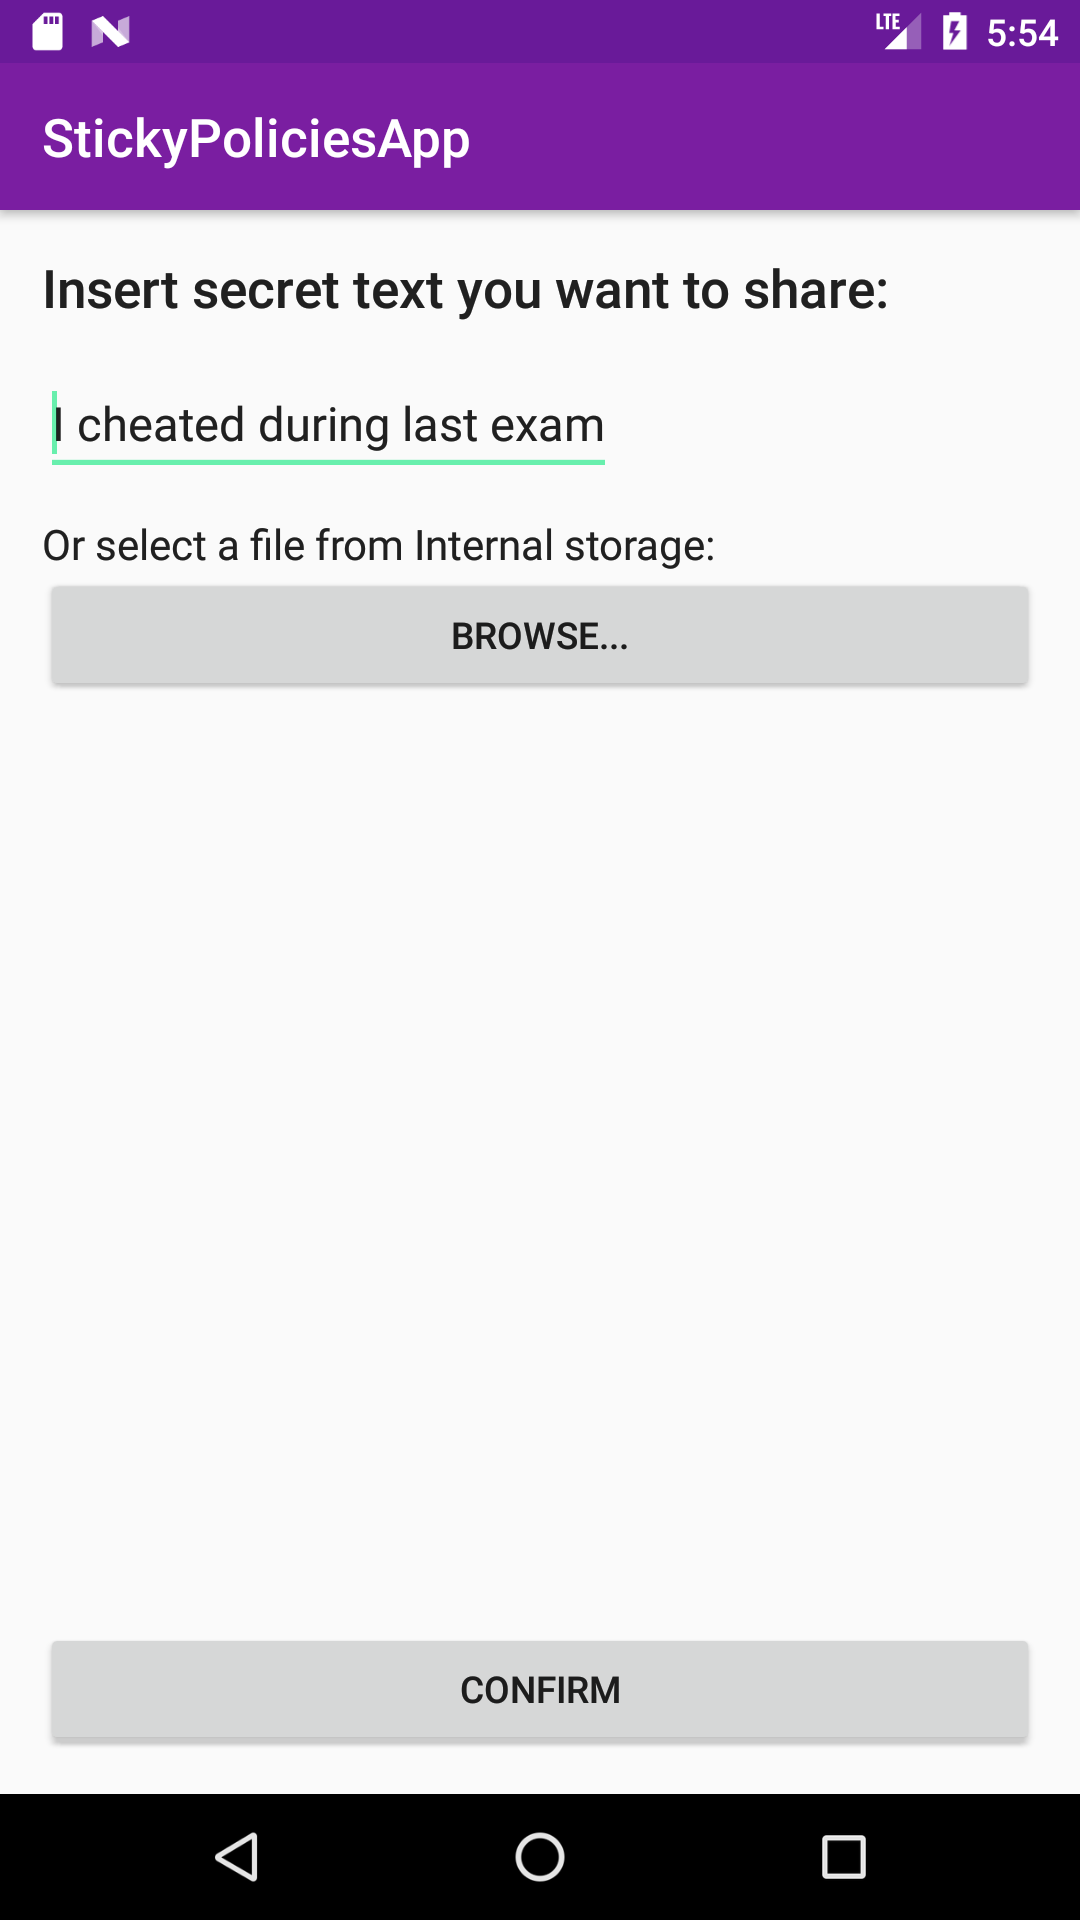
\includegraphics[width=0.9\textwidth]{ShareData-text.png} % first figure itself
		\caption{Sharing secret text}
		\label{fig:share-text}
	\end{minipage}
	\begin{minipage}{0.35\textwidth}
		\centering
		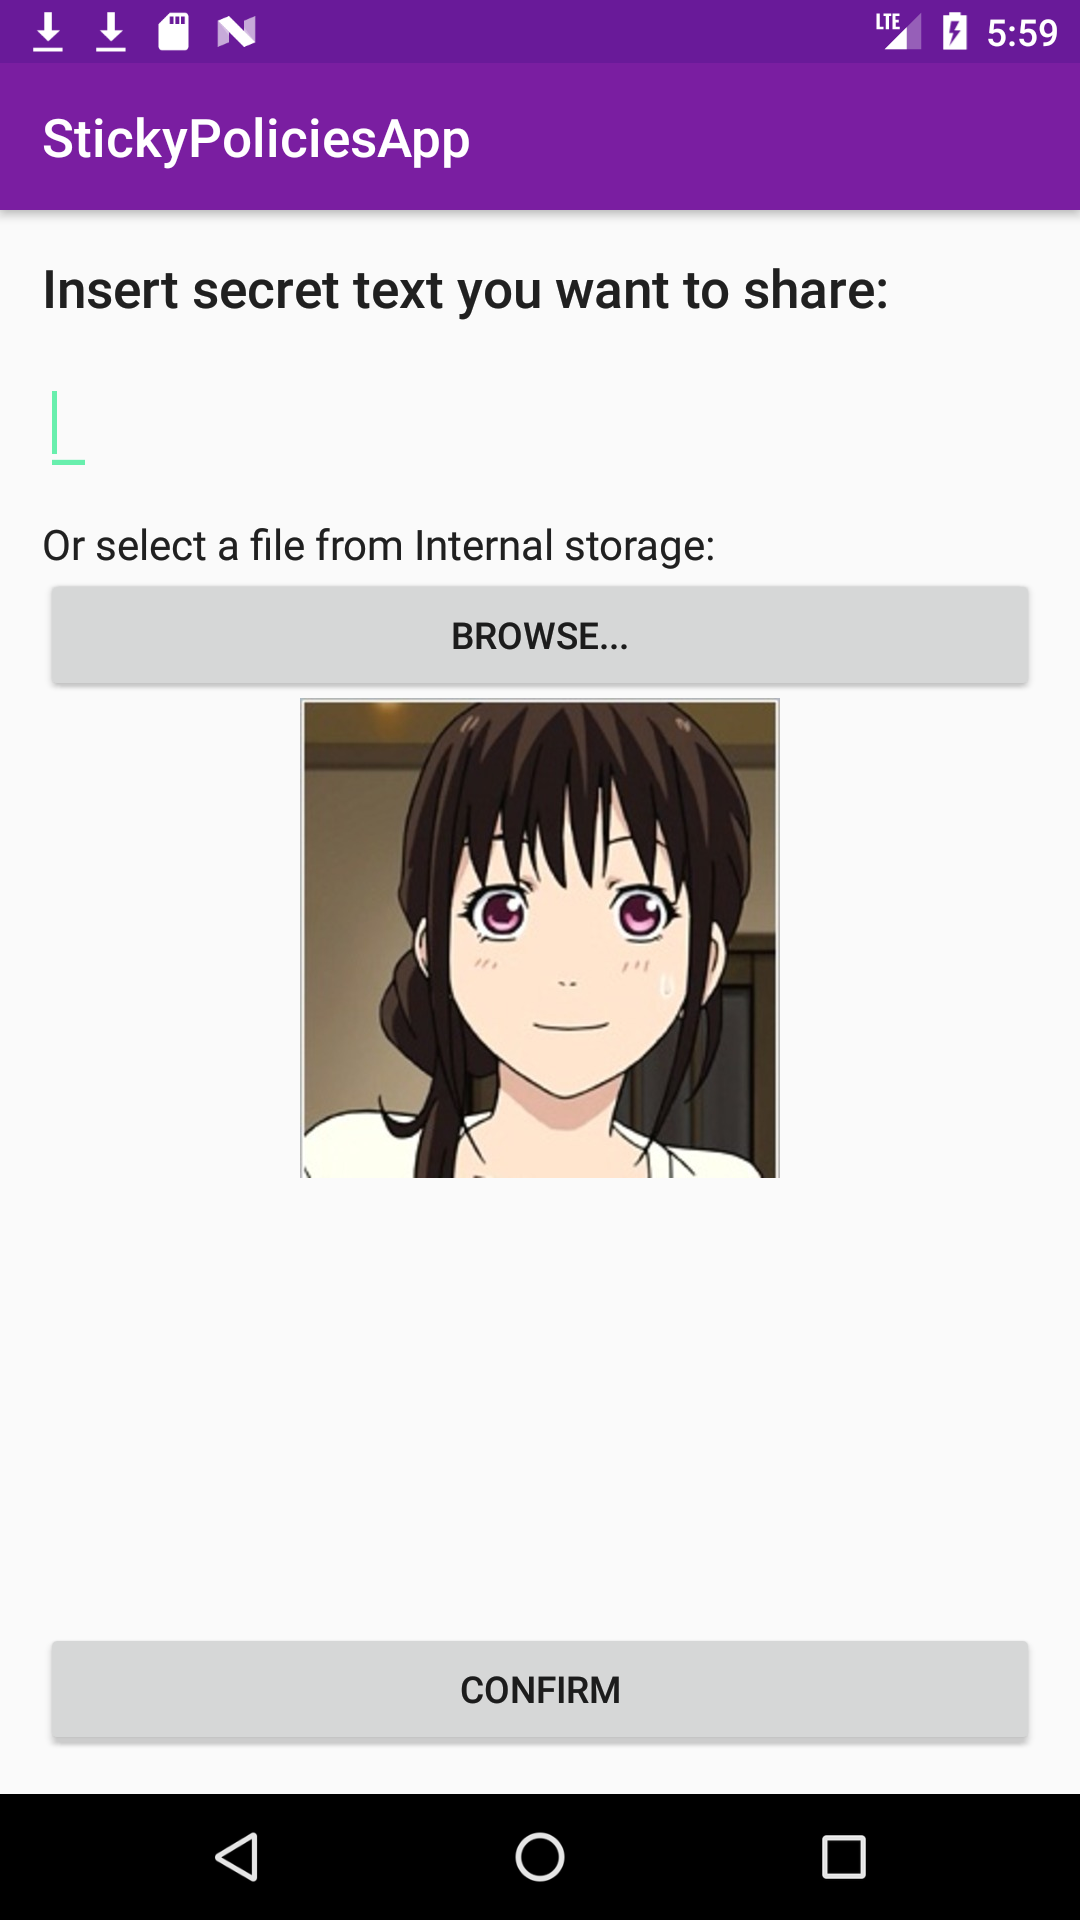
\includegraphics[width=0.9\textwidth]{ShareData-image.png} % second figure itself
		\caption{Sharing a personal image}
		\label{fig:share-img}
	\end{minipage}
\end{figure}


A certificate exchange is then initiated between the client and the server: this to perform both signature and encryption inside the app, and to allow the Trusted Authority to run security checks on data, when requested access by third parties. Subsequently, the policy and data are processed following the specification presented in \cite{mont2003towards}: the data is encrypted with a one-time-use symmetric key generated at the moment, and together with a digest of the policy they are first encrypted with the public key of the Trusted Authority, then signed with the data owner's private key.

It is now possible for Alice to safely share her data, sending it to Bob. Data is transferred inside the body of POST requests in JSON form. To safely and efficiently perform data serialization and deserialization we used the \texttt{com.google.code.gson} library and implemented an ad-hoc private class to hold both policy and encrypted data in a single JSON Object. For this purpose, we tested also the libraries \texttt{org.json} and \texttt{org.jabsorb}, which though proved to be unsuitable and less efficient.

Let's now consider the StickyPoliciesApp to be running on Bob's device, and to have just received a secret message from Alice. Bob forwards to the Trusted Authority the plaintext policy together with the signed key and digest, removing the encrypted personal data from the original payload. At this point, the Trusted Authority may check Bob's reliability and submit a few challenges to prove it, eventually disclosing the symmetric key to access Alice's secret message.

Both the communication and the cryptographic primitives are performed inside \texttt{AsyncTask}s to keep the main UI thread separated and responsive.

\subsection{Android Client Implementation}
The StickyPoliciesApp consists of a few \texttt{Activities}. The launcher allows both to send private data and to access received messages, but can be extended to include new functionalities, as the aforementioned policy editing.

Navigation within the activities is made through explicit \texttt{Intent}s: as specified within the Android Security guidelines, implicit \texttt{Intent}s may introduce security hazards as it is not known which service will respond to the intent, and the user has no control over it.

The first activity is in charge of data sharing: once the data type of the shared information is determined, it requests from the \texttt{CryptoUtils} class the data owner's certificate to retrieve its serial number, edits the sticky policy so that it matches both personal data type and certificate SN; finally, it creates a \texttt{Bundle} to pass these objects to the following activity, invoked explicitly.

The \texttt{PolicyClient} class is in charge of communication operations: it performs a certificate exchange with the Trusted Authority and it encrypts data, sending them to Bob. These operations are performed via dedicated \texttt{AsyncTask}s which are started in the \texttt{onResume()} method, so that the main UI thread is build without delay. Both tasks simply prepare data for the HTTP request, invoke a library function to handle it at a lower level and parse the results. For example, this is how the data owner's certificate is shared:
\lstinputlisting[caption={Excerpt from PolicyClient class},label={list:SendCert},language=java]{SendEncrData-excerpt.java}

\noindent where \texttt{NetworkUtils} is a public class exposing \texttt{static} methods for network management. As for data encryption, operations are performed following the specification in \cite{mont2003towards}, and an excerpt of the code is shown in Listing \ref{list:EncryptData}.
\lstinputlisting[caption={Excerpt from PolicyClient class},label={list:EncryptData},language=java]{SendEncrData-excerpt2.java}

In the above Listing, errors are handled via try-catch blocks for specific exceptions. To stop the application flow when a fatal error occurs (e.g. data decryption fails), a high-level exception is thrown with a message delivered to the user, who is prompted to retry the operation.

Finally, Bob can access the received data in a third \texttt{Activity}, in which he shares part of his \texttt{EncryptedData} with the Trusted Authority and receives back the symmetric key encrypted and the initialization vector.

\subsection{Java Server Implementation}

We have realized the Trusted Authority as a web server exposing two services, reachable via the corresponding servlets hosted in the servlet container Apache Tomcat.

The first one is in charge of sharing the Trusted Authority's \texttt{X509Certificate} in \texttt{PEM} format, and it also manages the data owners which want to register to the TA. Also in this case, the certificates are to be sent in \texttt{PEM} format. This state is kept server-side inside the \texttt{ServletContext}, which is bound to the servlet's life cycle rather to the single user or session.

The second service answers to data access requests: the servlet receives JSON Objects containing plaintext policies together with signed key and digest, and proceed checking the integrity of the policy, verifying the signature and decrypting the obtained data, to retrieve the symmetric key. If any of these procedures fails, the entire process is stopped and the access request is refused with an error code corresponding to the cause of the error (e.g. \texttt{403 Forbidden} in case the signature verification is not correct). In a future improved version of this app, the symmetric key could be encrypted with Bob's public key before sharing, requiring Bob to register at the Trusted Authority first. Other possible improvements include the implementation of policy-specified \texttt{action}s, as for example informing the data owner when data access is granted.

As it is, our web server shows the same weaknesses we described in the previous chapter; moreover, additional weaknesses are introduced by the communication with a potential malicious client. In other words, no check is performed on the payload (content-type, dimension, user-agent) and the client is considered to be always trusted.

\section{Structure of an XML policy}
The policy file is constructed by the data owner in order to specify which set of users can access her data. Policies are shared over the internet as strings, thus formats like XML or JSON represent the best choice in terms of interoperability and ease of use. Choosing the XML format over a new, custom implementation for Sticky Policies enables the use of well-known corroborated libraries and best practices, available due to XML widespread. Moreover, the document format is designed for data transfer and to be self-descriptive: its structure and content can easily be regulated through grammars and specifications.

Sticky Policies have been designed with a general and comprehensive structure, so as to allow broader usage than the one proposed in this solution. The main components of a Sticky Policy are the following:
\begin{itemize}
	\item List of the Trusted Authorities in which Bob can ask for data access. They are specified by Alice and they include all the servers in which she registered her certificate.
	\item Details about the Data Owner, which are used server-side to retrieve the correct certificate and public key.
	\item One or more policy, specifying fine-grained constraints about the attached data. They may vary in target, time validity, requirements, etc.; the complete specification is available in Appendix \ref{appendixA}.
\end{itemize}

\subsection{XML Validation and Parsing}
Policies are parsed server side: this control step includes validation, i.e. checking both syntax and semantics of the document. In Java, it is possible to realize an XML parser through a \texttt{SAXParser}: this low-level implementation scans the whole document and for each start tag and end tag found fires and event, handled by a callback method to retrieve the content between the tags. While this allows to gain in efficiency and is suited also to parse large documents, it constitutes and ad-hoc tailored solution, unsuited for dynamic environments.

Document parsing is performed by a \texttt{ContentHandler}, in which callback methods are defined: we chose to implement them via the subclass \texttt{DefaultHandler} and its methods \texttt{startElement}, \texttt{characters}, \texttt{endElement}.

In our solution, we implemented also a \texttt{XMLErrorChecker} for error handling. This parser provides three different types of errors: fatal errors, errors and warnings, although by default only fatal errors are fired. In these cases, the parser cannot continue parsing and the method performs \texttt{System.exit(1)}, while nonfatal errors are generated when the document fails some validity constraints (e.g. invalid tag, tag not allowed...). We redefined the default behaviour by firing \texttt{SAXException}s also for nonfatal errors, due to the considerable importance of having a well-formed and valid document. These exceptions are then catched by the caller, at a higher level of the call stack, and handled by refusing the data disclosure request.


\section{About cryptography}
Cryptography constitutes a considerable part of the whole project. All cryptographic functions are realized as static, and accessible as if they were an external library both in the client and server. Both of them rely on the Java Cryptography Architecture together with Bouncy Castle APIs.

\subsection{X509Certificates}
The Bouncy Castle library provides functionalities to create self-signed X509 Certificates, chosen for the sake of simplicity. In a more realistic implementation, certificates should be issued by a Certification Authority, and the web server should additionally perform certificate verification (e.g. expiration and revocation). To construct the \texttt{X509Certificate}, we use 1024-bit asymmetric keys generated for the RSA algorithm, and the Bouncy Castle security provider. 2048-bit long keys could be more appropriate depending on the confidentiality of the information shared, on the mobile device and network possibilities.

Both the certificates are constructed following the same instructions. In case the Trusted Authority works also as a Certification Authority, then 

\lstinline[language=java]!BasicConstraints constraints = new BasicConstraints(true);!

while for the mobile device we use a \texttt{false} parameter. Moreover, in both cases, certificates are created and handled as singleton objects, to prevent inappropriate certificate creation: the methods and fields to generate and store certificates are \texttt{private}, and their content can be retrieved through accessor methods, which also control the instance creation.

Among the Bouncy Castle library there is the LightCrypto implementation \cite{LightCrypto}, available for phones or devices with limited computational power. It allows the creation of key pairs and certificates, but their interoperability with the Java Cryptography Architecture is limited so that a conventional certificate implementation is preferred. 

Certificates are shared in PEM format using a \texttt{JcaPEMWriter} for serialization and a \texttt{CertificateFactory} for deserialization. This format has been preferred to ASN.1 as easier to send in a HTML request body, it being a \texttt{String} rather than a \texttt{byte[]}.

\subsection{Message Digests}
Computing message digests is an important part of this security protocol: first, it proves policy's integrity by matching the received digest with the one computed from the plaintext policy; second, it lowers the size of the data to be encrypted, giving it a fixed dimension of 32 bytes. In fact, policy files can potentially grow in size and, were the policy not to be hashed before asymmetric encryption, it could introduce a weakness within RSA's encryption method. If the overall dimension of the symmetric key and policy were greater than the dimension of the modulus for asymmetric encryption, either the dimension of the modulus would increase, or encryption would be performed after splitting the whole data into blocks of size lower than 1024 bits.

The cryptographic hash function used in this project is the SHA-256 function, and the implementation is the one provided by the class \texttt{java.security. MessageDigest}. To obtain a message digest it is necessary to follow a three-step procedure: first, an instance of \texttt{MessageDigest} is retrieved for the specific algorithm; then, it receives as input the text to hash and, finally, the \texttt{digest()} function is called.

\lstinputlisting[caption={Excerpt from CryptoUtilities class},label={list:MessageDigest},language=java]{MessageDigest.java}

Digests are compared with the \texttt{MessageDigest.isEqual(byte[] first, byte[] second)} function, which does a simple byte compare, as reported by the Java documentation.

Switching from SHA-256 to SHA-512 could increase efficiency in our case, thanks to the chosen device having a x86\_64 architecture and being SHA-512 based on 64-bits words.  Furthermore, this would not pose any problem in terms of API availability since both of them are available since API level 1+. Switching to SHA-512 would double the size of the produced digest, leaving only 64 bytes of space to encode the symmetric key. Keeping into consideration previous observations about having a maximum data size of 128 bytes, we have preferred a smaller message digest also in terms of bandwith consumption and foreseeing a possible symmetric-key dimension increase.

\subsection{Symmetric Key Generation and Encryption}
In this subsection, we will refer always to cryptographic operations happening on the Android devices, since the Trusted Authority never receives personal data.

The specification in paper \cite{mont2003towards} asks for a symmetric one-time-use key to encode personal data. Symmetric keys can be generated via a \texttt{KeyGenerator} with an algorithm-specific initialization, not providing \texttt{SecureRandom} to rely on the implementation of the highest-priority installed provider. This raises the reliability of the proposed solution, as symmetric keys are never reused and are unrelated. The available algorithms for encryption and key generation depend on the chosen security \texttt{Provider}, which is in our case the Bouncy Castle provider. Available key generation algorithms include AES for symmetric encryption, but it is only possible to use is with AES/ECB or AES/GCM/NOPADDING: since the former has known weaknesses and it is not suited to large-size files encryption, we considered the second method. A working example is shown in Listing \ref{list:ECBencryption}.

Buoncy Castle also offers implementations for several Password Based Encryption methods, using AES/CBC with different key lengths, salt and padding options. We did not consider any of those algorithms as they are out of the scope of this project: encryption must be performed with a one-time-use secret, while using a fixed password would definitely reduce the security level. Moreover, PBE requires many iterations in order to process a secure derived key (around 100 000 or 200 000), which could impact on efficiency and performance.

\lstinputlisting[caption={Example code with ECB encryption on Android device},label={list:ECBencryption},language=java]{EncryptSymmetricECB.java}

Alternatively, a AES\_256/CBC/PKCS7Padding  algorithm is available with the AndroidOpenSSL provider: the Cipher Block Chaining algorithm is more secure than Electronic Codebook, and is suited to work in this context as a block cipher mode. Padding is needed due to unpredictable size of the policy, which may not be a multiple of the block size (128 bits).

To implement this solution we need to provide an initialization vector to be XORed with the first block of plaintext: to obtain it we rely on the Java class \texttt{SecureRandom}, and we create it with the same size of block in CBC. In this case, when creating a symmetric key we just need to specify \texttt{"AES"} as input parameter, while for the encryption and decryption methods we add a initialization vector:

\lstinputlisting[caption={Example code with CBC encryption on Android device},label={list:CBCencryption},language=java]{EncryptSymmetricCBC.java}

From the code in Listing \ref{list:CBCencryption} descends immediately that it is impossible to share data with this encryption algorithm, due to the need of initialization vectors. It is useful to observe the result of Bob's decryption of Alice's secret data "I cheated during last exam", as shown in Figure \ref{fig:DecryptCBCInvalidIV}

\begin{figure}
	\centering
	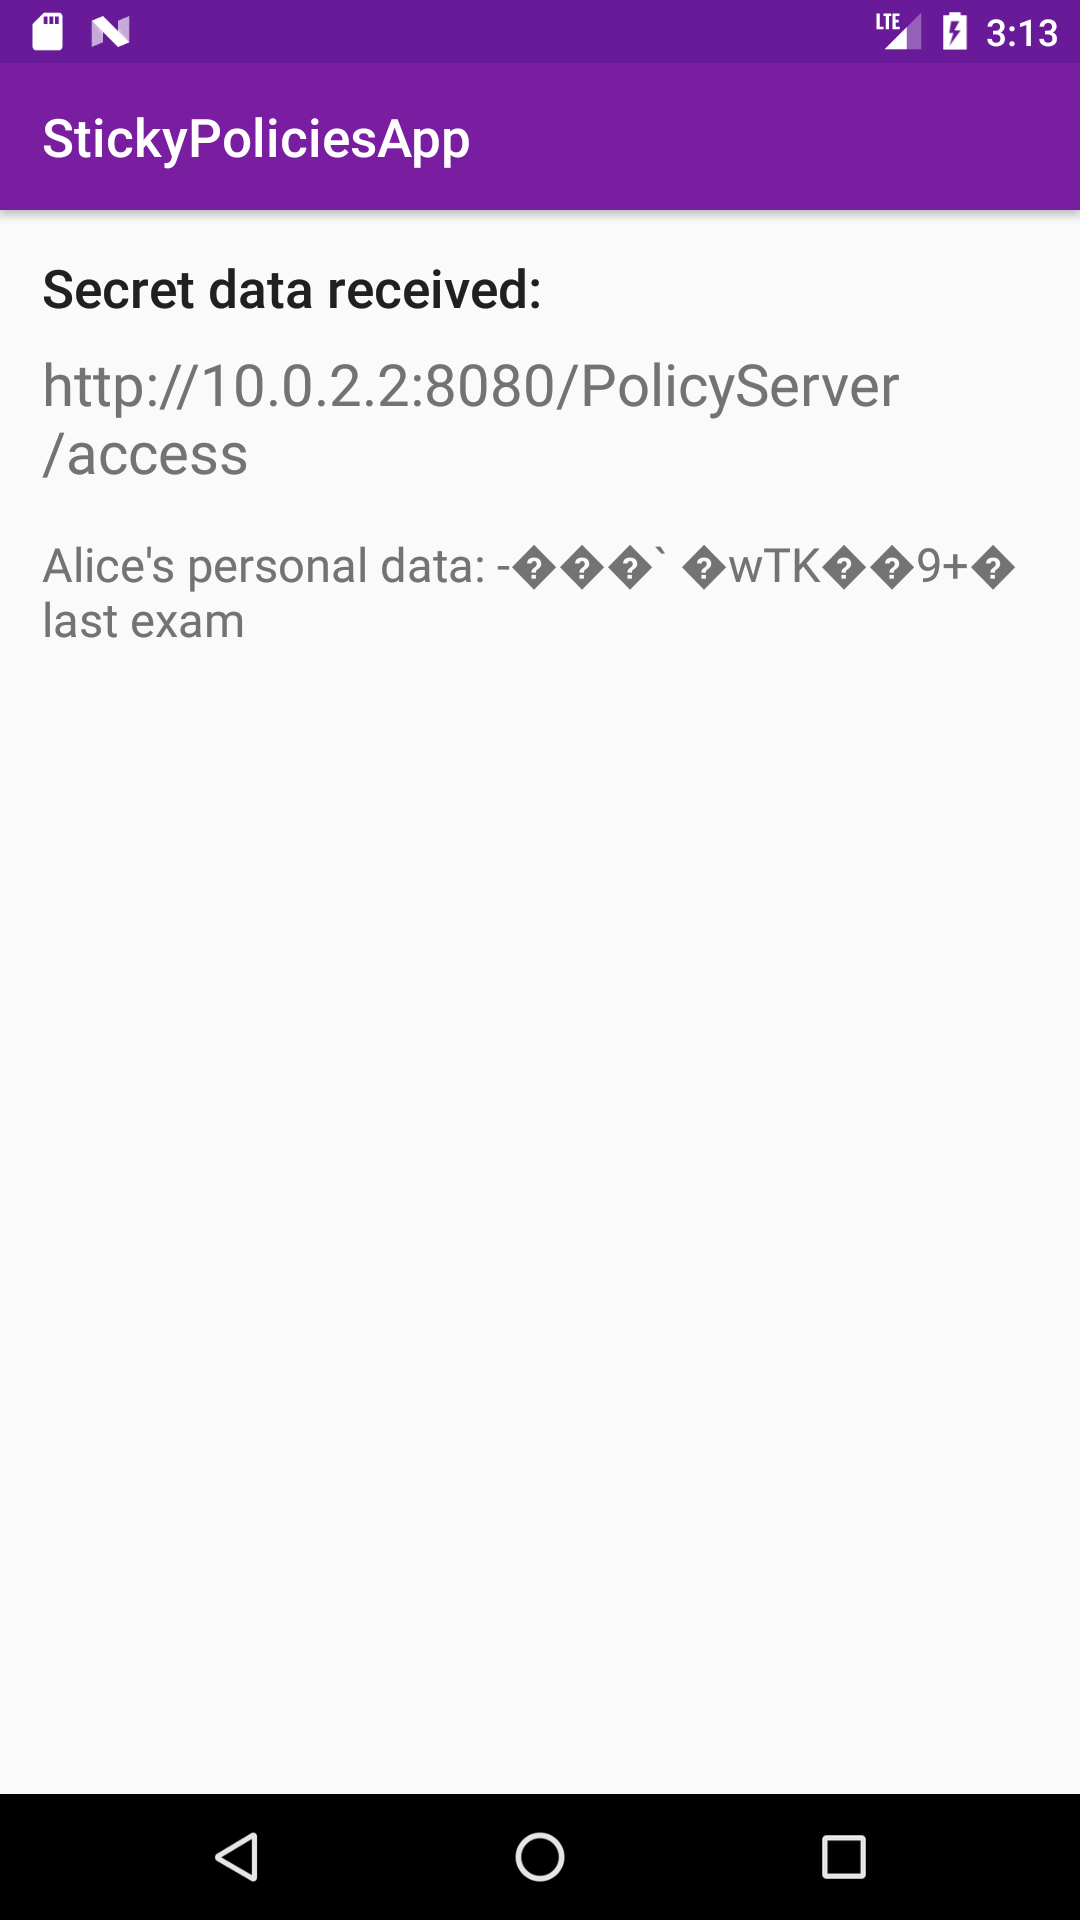
\includegraphics[width=0.35\linewidth]{DecryptCBCInvalidIV.png}
	\caption{Decrypted text in Bob's device.}
	\label{fig:DecryptCBCInvalidIV}
\end{figure}

In the decrypted text, the first part of the text is wrong, while the second part can be understood. This is because if the IV is not shared or is incorrect, the receiver will still be able to understand the message. Consequently, to use CBC it should be necessary to share also the initialization vector together with the secret key to encrypt the whole message properly. In other words, this introduces another weakness in the message protocol, because a potential attacker would only need to get hold of the key to encrypt information, instead of both key and initialization vector.


symmetric key generation, symmetric key algorithm for encryption

initialization vector

sign, verify, encrypt and decrypt with asymmetric keys

performance of the whole process, padding, salt, random generation in android


\section{Performance}


